\section{Installation}

%%%%%%%%%%%%%%%%%%%%%%%%%%%%%%%%%%%%%%%%%%%%%%%%%%%%%%%%%%%%%%%%%%%%%%%%%%%%%%%%

\begin{frame}[fragile]{Architecture}

\begin{figure}
\begin{center}
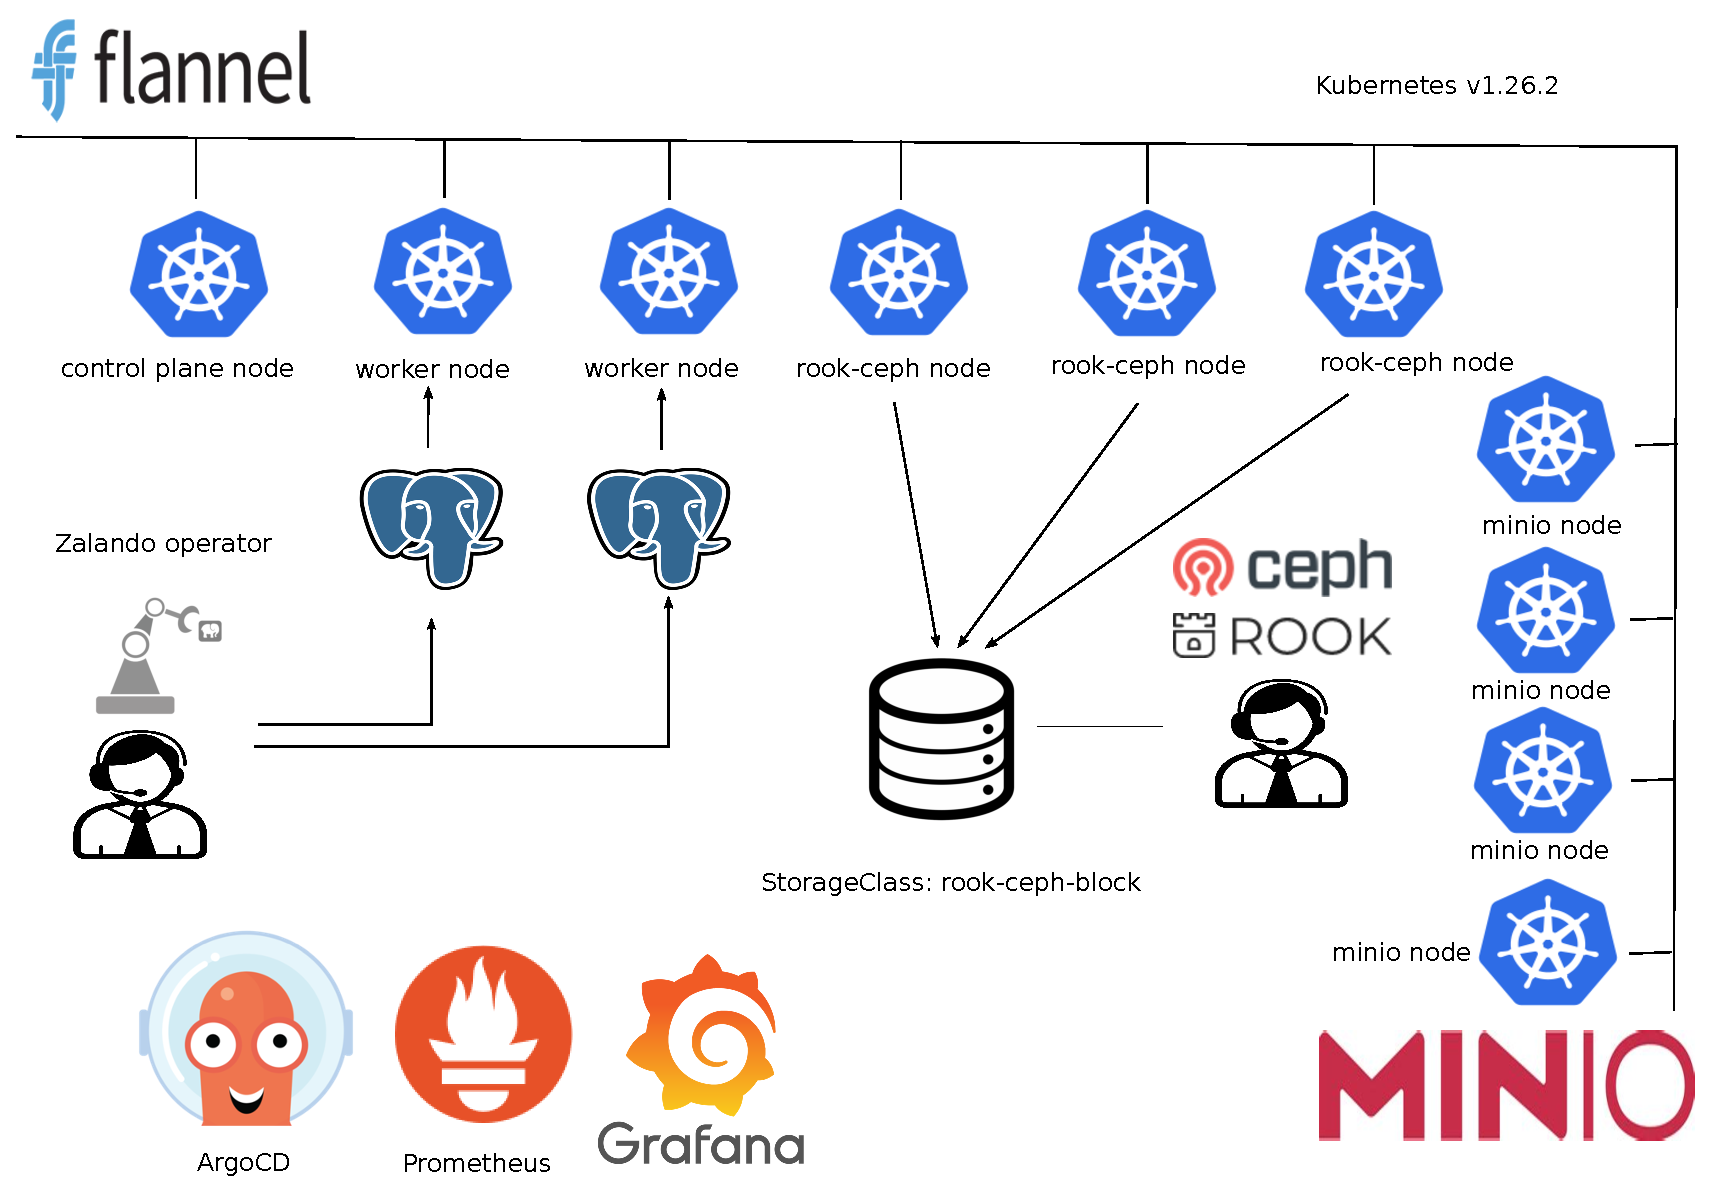
\includegraphics[scale=0.5]{images/architecture.eps}
\end{center}
\end{figure}

\end{frame}

%%%%%%%%%%%%%%%%%%%%%%%%%%%%%%%%%%%%%%%%%%%%%%%%%%%%%%%%%%%%%%%%%%%%%%%%%%%%%%%%

\begin{frame}[fragile]{Versions utilisées}

   \begin{itemize}
      \item OS de déploiement: Debian 11 - Bullseye
      \item Versions de Kubernetes: 1.26.x
   \end{itemize}

\end{frame}

%%%%%%%%%%%%%%%%%%%%%%%%%%%%%%%%%%%%%%%%%%%%%%%%%%%%%%%%%%%%%%%%%%%%%%%%%%%%%%%%

\begin{frame}[fragile]{Déploiement du n{\oe}ud \textbf{control plane}}

   \begin{itemize}
      \item Kubernetes s'appuie sur un élément essentiel qui est le \textit{container runtime}.
      \item La méthode de déploiement du container runtime s'appuie la méthode décrite dans le lien: \url{https://docs.docker.com/engine/install/debian/}
   \end{itemize}

\begin{tiny}
\begin{Verbatim}[commandchars=\\\{\}]
\end{Verbatim}
\end{tiny}


\end{frame}

%%%%%%%%%%%%%%%%%%%%%%%%%%%%%%%%%%%%%%%%%%%%%%%%%%%%%%%%%%%%%%%%%%%%%%%%%%%%%%%%

\begin{frame}[fragile]{Installation du runtine container \textit{containerd}}

Mise à jour de l'index du paquet \textit{apt} et installation des paquets nécessaires à l'utilisation des dépôts avec le protocole HTTPS:

\begin{tiny}
\begin{Verbatim}[commandchars=\&\#\#]
sudo apt-get update

sudo apt-get install \
    ca-certificates \
    curl \
    gnupg

\end{Verbatim}
\end{tiny}

\end{frame}

%%%%%%%%%%%%%%%%%%%%%%%%%%%%%%%%%%%%%%%%%%%%%%%%%%%%%%%%%%%%%%%%%%%%%%%%%%%%%%%%

\begin{frame}[fragile]{Ajout de la clef GPG officielle de Docker}

\begin{tiny}
\begin{Verbatim}[commandchars=\&\#\#]
sudo install -m 0755 -d /etc/apt/keyrings
curl -fsSL https://download.docker.com/linux/debian/gpg | sudo gpg --dearmor -o /etc/apt/keyrings/docker.gpg
sudo chmod a+r /etc/apt/keyrings/docker.gpg
\end{Verbatim}
\end{tiny}

\end{frame}

%%%%%%%%%%%%%%%%%%%%%%%%%%%%%%%%%%%%%%%%%%%%%%%%%%%%%%%%%%%%%%%%%%%%%%%%%%%%%%%%

\begin{frame}[shrink=7,fragile]{Ajout du dépôt de Docker}

\begin{tiny}
\begin{Verbatim}[commandchars=\&\#\#]
  echo \
  "deb [arch="$(dpkg --print-architecture)" signed-by=/etc/apt/keyrings/docker.gpg] https://download.docker.com/linux/debian \
  "$(. /etc/os-release && echo "$VERSION_CODENAME")" stable" | \
  sudo tee /etc/apt/sources.list.d/docker.list > /dev/null
\end{Verbatim}
\end{tiny}

\end{frame}

%%%%%%%%%%%%%%%%%%%%%%%%%%%%%%%%%%%%%%%%%%%%%%%%%%%%%%%%%%%%%%%%%%%%%%%%%%%%%%%%

\begin{frame}[fragile]{Installation de Docker Engine}

\begin{tiny}
\begin{Verbatim}[commandchars=\&\#\#]
   sudo apt-get update
   sudo apt-get install docker-ce docker-ce-cli containerd.io docker-buildx-plugin docker-compose-plugin
\end{Verbatim}
\end{tiny}

\end{frame}

%%%%%%%%%%%%%%%%%%%%%%%%%%%%%%%%%%%%%%%%%%%%%%%%%%%%%%%%%%%%%%%%%%%%%%%%%%%%%%%%

\begin{frame}[shrink=7,fragile]{Installation de \textbf{kubectl, kubeadm et kubelet}}

\begin{tiny}
\begin{Verbatim}[commandchars=\&\#\#]
sudo curl -fsSLo /etc/apt/keyrings/kubernetes-archive-keyring.gpg https://packages.cloud.google.com/apt/doc/apt-key.gpg
echo "deb [signed-by=/etc/apt/keyrings/kubernetes-archive-keyring.gpg] https://apt.kubernetes.io/ kubernetes-xenial main" | \
sudo tee /etc/apt/sources.list.d/kubernetes.list

sudo apt-get update
sudo apt-get install -y kubectl
sudo apt-get install -y kubeadm
sudo apt-get install -y kubelet
\end{Verbatim}
\end{tiny}

\end{frame}

%%%%%%%%%%%%%%%%%%%%%%%%%%%%%%%%%%%%%%%%%%%%%%%%%%%%%%%%%%%%%%%%%%%%%%%%%%%%%%%%

\begin{frame}[fragile]{Activation des modules kernel \textit{overlay} et \textit{br\_netfilter}}

\begin{tiny}
\begin{Verbatim}[commandchars=\&\#\#]
linagora@debian-cp:/etc/modules-load.d$ cat k8s.conf 
overlay
br_netfilter
linagora@debian-cp:/etc/modules-load.d$ pwd
/etc/modules-load.d
\end{Verbatim}
\end{tiny}

\end{frame}

%%%%%%%%%%%%%%%%%%%%%%%%%%%%%%%%%%%%%%%%%%%%%%%%%%%%%%%%%%%%%%%%%%%%%%%%%%%%%%%%

\begin{frame}[fragile]{Activation des fonctions \textit{bridge/iptables} et \textit{forward} du kernel}

\begin{tiny}
\begin{Verbatim}[commandchars=\&\#\#]
linagora@debian-cp:/etc/sysctl.d$ cat k8s.conf 
inet.bridge.bridge-nf-call-iptables  = 1
net.bridge.bridge-nf-call-ip6tables = 1
net.ipv4.ip_forward                 = 1
linagora@debian-cp:/etc/sysctl.d$ pwd
/etc/sysctl.d
\end{Verbatim}
\end{tiny}

\end{frame}

%%%%%%%%%%%%%%%%%%%%%%%%%%%%%%%%%%%%%%%%%%%%%%%%%%%%%%%%%%%%%%%%%%%%%%%%%%%%%%%%

\begin{frame}[fragile]{Paramétrage de containerd}

Génération du paramétrage par défaut de containerd:

\begin{tiny}
\begin{Verbatim}[commandchars=\\\{\}]
root@debian-cp:~# containerd config \userinput{default} dump > /etc/containerd/config.toml.dmp
\end{Verbatim}
\end{tiny}

Modifier la valeur à \textbf{true} pour le paramètre \textbf{SystemdCgroup}:

\begin{tiny}
\begin{Verbatim}[commandchars=\\\{\}]
[plugins."io.containerd.grpc.v1.cri".containerd.runtimes.runc.options]
  BinaryName = ""
  CriuImagePath = ""
  CriuPath = ""
  CriuWorkPath = ""
  IoGid = 0
  IoUid = 0
  NoNewKeyring = false
  NoPivotRoot = false
  Root = ""
  ShimCgroup = ""
  SystemdCgroup = \userinput{true}
\end{Verbatim}
\end{tiny}

\end{frame}

%%%%%%%%%%%%%%%%%%%%%%%%%%%%%%%%%%%%%%%%%%%%%%%%%%%%%%%%%%%%%%%%%%%%%%%%%%%%%%%%

\begin{frame}[fragile]{Paramétrage de containerd}

Remplacer le paramétrage actuel par le paramétrage modifié:

\begin{tiny}
\begin{Verbatim}[commandchars=\\\{\}]
root@debian-cp:~# cp /etc/containerd/config.toml /etc/containerd/config.toml.bak
root@debian-cp:~# cat /etc/containerd/config.toml.dmp > /etc/containerd/config.toml
root@debian-cp:~# systemctl restart containerd
\end{Verbatim}
\end{tiny}

\end{frame}

%%%%%%%%%%%%%%%%%%%%%%%%%%%%%%%%%%%%%%%%%%%%%%%%%%%%%%%%%%%%%%%%%%%%%%%%%%%%%%%%

\begin{frame}[fragile]{Initialisation du cluster Kubernetes}

En tant que root, lancer la commande suivante:

\begin{tiny}
\begin{Verbatim}[commandchars=\&\@\@]
# kubeadm init --control-plane-endpoint 10.10.10.30 \
--skip-phases=addon/coredns,addon/kube-proxy \
--v=5 \
--pod-network-cidr="10.244.0.0/16"
\end{Verbatim}
\end{tiny}

Si les phases \textit{addon/coredns} et \textit{addon/kube-proxy} ne sont pas évitées au $1^{er}$ lancement de kubeadm, l'erreur suivante est générée:

\begin{toile}
[kubelet-finalize] Updating "/etc/kubernetes/kubelet.conf" to point to a rotatable kubelet client certificate and key
error execution phase addon/coredns: unable to fetch CoreDNS current installed version and ConfigMap.: rpc error: code = Unknown desc = malformed header: missing HTTP content-type
To see the stack trace of this error execute with --v=5 or higher
\end{toile}

\end{frame}

%%%%%%%%%%%%%%%%%%%%%%%%%%%%%%%%%%%%%%%%%%%%%%%%%%%%%%%%%%%%%%%%%%%%%%%%%%%%%%%%

\begin{frame}[shrink=7,fragile]{Initialisation du cluster Kubernetes}

Le résultat de la commande d'init est le suivant:

\begin{toile}

I0315 01:06:38.342010   34405 kubeletfinalize.go:134] [kubelet-finalize] Restarting the kubelet to enable client certificate rotation\\
\\
Your Kubernetes control-plane has initialized successfully!\\
\\
To start using your cluster, you need to run the following as a regular user:

\begin{tiny}
\begin{Verbatim}[commandchars=\&\@\@]
  mkdir -p $HOME/.kube
  sudo cp -i /etc/kubernetes/admin.conf $HOME/.kube/config
  sudo chown $(id -u):$(id -g) $HOME/.kube/config
\end{Verbatim}
\end{tiny}

Alternatively, if you are the root user, you can run:\\

\begin{tiny}
\begin{Verbatim}[commandchars=\&\@\@]
  export KUBECONFIG=/etc/kubernetes/admin.conf
\end{Verbatim}
\end{tiny}

You should now deploy a pod network to the cluster.\\
Run "kubectl apply -f [podnetwork].yaml" with one of the options listed at:\\
  https://kubernetes.io/docs/concepts/cluster-administration/addons/

You can now join any number of control-plane nodes by copying certificate authorities
and service account keys on each node and then running the following as root:

\begin{tiny}
\begin{Verbatim}[commandchars=\&\@\@]
  kubeadm join 10.10.10.30:6443 --token 6pia7c.n6u8pbm7yjl6nnr8 \
        --discovery-token-ca-cert-hash sha256:f6d45602ea75c7659dc91f661d19e97e6817e2847e4e5d0047880b871317a145 \
        --control-plane 
\end{Verbatim}
\end{tiny}

Then you can join any number of worker nodes by running the following on each as root:

\begin{tiny}
\begin{Verbatim}[commandchars=\&\@\@]
kubeadm join 10.10.10.30:6443 --token 6pia7c.n6u8pbm7yjl6nnr8 \
        --discovery-token-ca-cert-hash sha256:f6d45602ea75c7659dc91f661d19e97e6817e2847e4e5d0047880b871317a145 
\end{Verbatim}
\end{tiny}

\end{toile}

\end{frame}

%%%%%%%%%%%%%%%%%%%%%%%%%%%%%%%%%%%%%%%%%%%%%%%%%%%%%%%%%%%%%%%%%%%%%%%%%%%%%%%%

\begin{frame}[fragile]{Paramétrage de \textit{kubectl}}

   L'utilisation de kubectl nécessite l'action suivante:

\begin{tiny}
\begin{Verbatim}[commandchars=\&\@\@]
  mkdir -p $HOME/.kube
  sudo cp -i /etc/kubernetes/admin.conf $HOME/.kube/config
  sudo chown $(id -u):$(id -g) $HOME/.kube/config
\end{Verbatim}
\end{tiny}

\end{frame}

%%%%%%%%%%%%%%%%%%%%%%%%%%%%%%%%%%%%%%%%%%%%%%%%%%%%%%%%%%%%%%%%%%%%%%%%%%%%%%%%

\begin{frame}[fragile]{Déploiement de l'addon \textbf{CoreDNS}}

   Comme indiqué précédemment, les addons CoreDNS et Kube-Proxy n'ont pas été déployés au $1^{er}$ lancement de kubeadm.\\
   CoreDNS peut maintenant être déployé sans erreur:\\

\begin{tiny}
\begin{Verbatim}[commandchars=\\\{\}]
linagora@debian-cp:~$ sudo kubeadm init phase addon coredns
[addons] Applied essential addon: CoreDNS
\end{Verbatim}
\end{tiny}

\end{frame}

%%%%%%%%%%%%%%%%%%%%%%%%%%%%%%%%%%%%%%%%%%%%%%%%%%%%%%%%%%%%%%%%%%%%%%%%%%%%%%%%

\begin{frame}[fragile]{Déploiement de l'addon \textbf{Kube-Proxy}}

\begin{tiny}
\begin{Verbatim}[commandchars=\\\{\}]
linagora@debian-cp:~$ sudo kubeadm init phase addon kube-proxy
[addons] Applied essential addon: kube-proxy
\end{Verbatim}
\end{tiny}

\end{frame}

%%%%%%%%%%%%%%%%%%%%%%%%%%%%%%%%%%%%%%%%%%%%%%%%%%%%%%%%%%%%%%%%%%%%%%%%%%%%%%%%

\begin{frame}[fragile]{Choix de la couche réseau - \textbf{Container Network Interface}}

   Il existe différentes addons Kubernetes implémentant l'interface CNI.\\
   Ces addons sont listés dans l'URL suivante: \url{https://kubernetes.io/docs/concepts/cluster-administration/addons/}\\
   Pour le POC, l'addon sélectionné est Flannel car il semble être le plus simple et le plus basique des addons CNI.\\

\end{frame}

%%%%%%%%%%%%%%%%%%%%%%%%%%%%%%%%%%%%%%%%%%%%%%%%%%%%%%%%%%%%%%%%%%%%%%%%%%%%%%%%

\begin{frame}[fragile]{Déploiement de l'addon \textit{Flannel}}

   L'addon Flannel s'installe de plusieurs manières (\url{https://github.com/flannel-io/flannel#deploying-flannel-manually}).\\
   La méthode utilisée pour le POC est kubectl:

\begin{tiny}
\begin{Verbatim}[commandchars=\\\{\}]
kubectl apply -f https://github.com/flannel-io/flannel/releases/latest/download/kube-flannel.yml
\end{Verbatim}
\end{tiny}

\end{frame}

%%%%%%%%%%%%%%%%%%%%%%%%%%%%%%%%%%%%%%%%%%%%%%%%%%%%%%%%%%%%%%%%%%%%%%%%%%%%%%%%

\begin{frame}[fragile]{Installation de \textbf{k9s}}

   Un outil pratique de visualisation d'un cluster kubernetes est: \textbf{k9s} (\url{https://k9scli.io/})\\
   Le lien suivant permet de télécharger l'archive incluant le binaire: \url{https://github.com/derailed/k9s/releases/download/v0.27.3/k9s_Linux_amd64.tar.gz}


\end{frame}

%%%%%%%%%%%%%%%%%%%%%%%%%%%%%%%%%%%%%%%%%%%%%%%%%%%%%%%%%%%%%%%%%%%%%%%%%%%%%%%%

\begin{frame}[fragile]{Liste des namespaces}

\begin{tiny}
\begin{Verbatim}[commandchars=\\\{\}]
linagora@debian-cp:~$ kubectl get namespaces
NAME              STATUS   AGE
default           Active   40d
kube-flannel      Active   39d
kube-node-lease   Active   40d
kube-public       Active   40d
kube-system       Active   40d
minio-operator    Active   32d
rook-ceph         Active   32d
\end{Verbatim}
\end{tiny}

\begin{figure}
\begin{center}
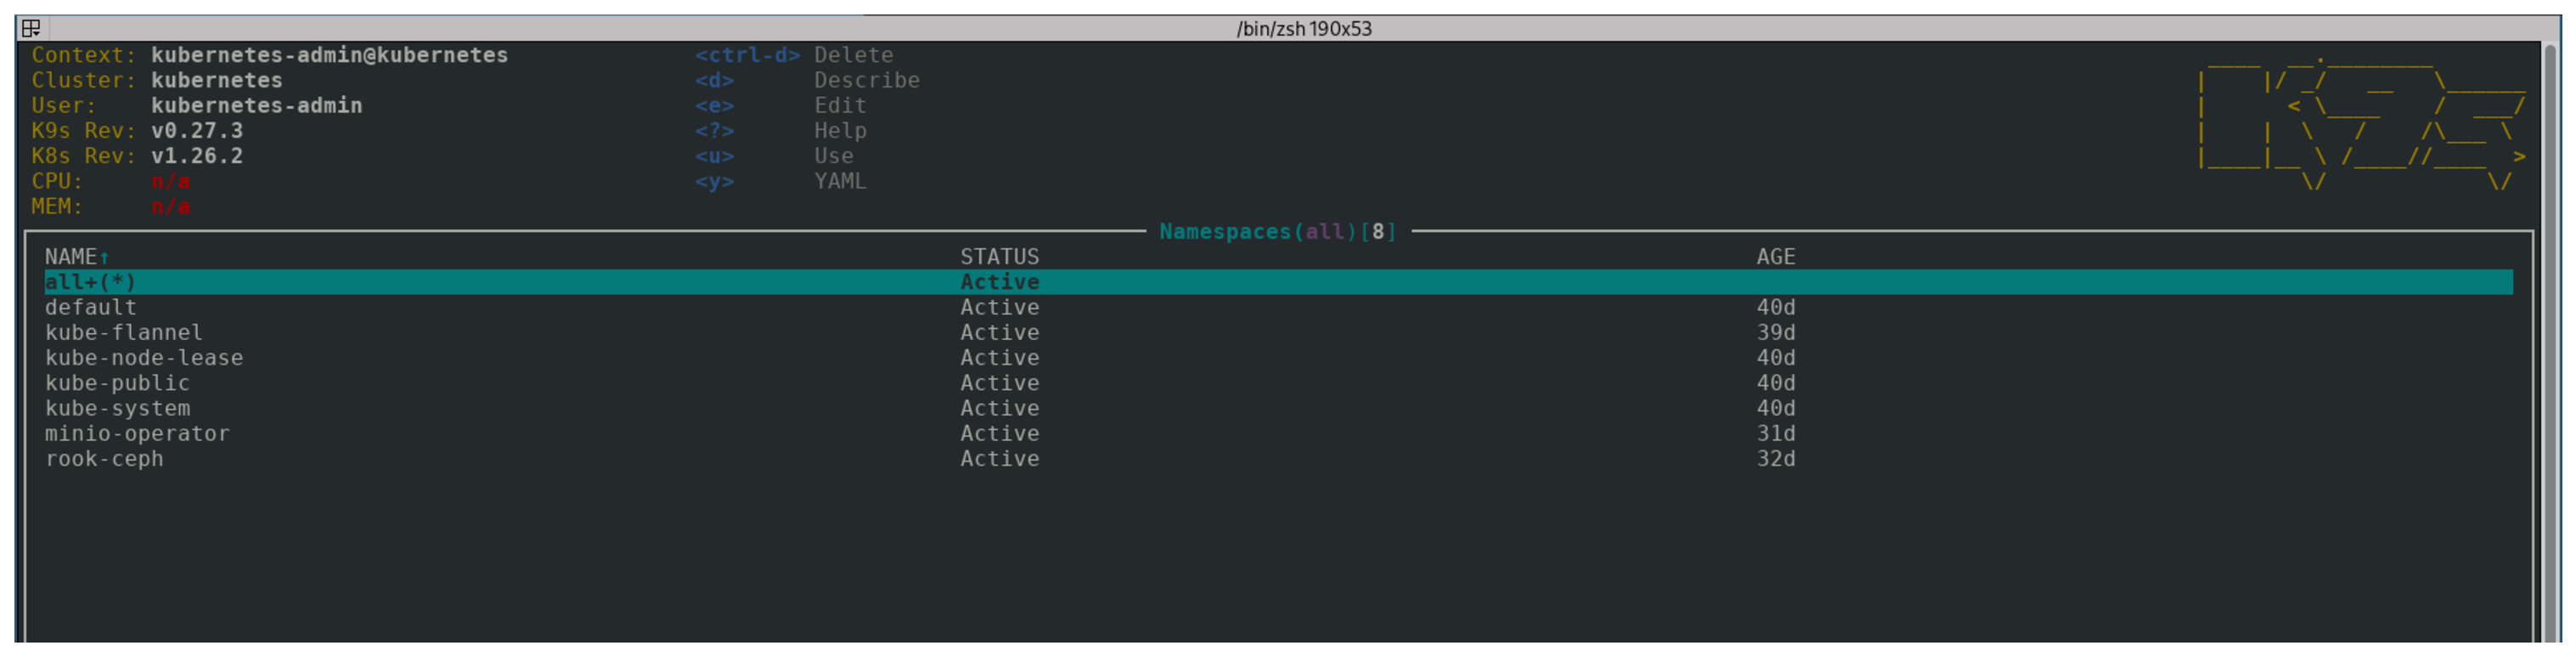
\includegraphics[angle=0, width=0.5\textwidth]{namespaces.eps}
\end{center}
\end{figure}

\end{frame}

%%%%%%%%%%%%%%%%%%%%%%%%%%%%%%%%%%%%%%%%%%%%%%%%%%%%%%%%%%%%%%%%%%%%%%%%%%%%%%%%

\begin{frame}[fragile]{Pods du namespace default}

\begin{tiny}
\begin{Verbatim}[commandchars=\\\{\}]
linagora@debian-cp:~$ kubectl get pods          
NAME                                    READY   STATUS    RESTARTS   AGE
acid-test-cluster-0                     1/1     Running   0          27d
acid-test-cluster-1                     1/1     Running   0          27d
postgres-operator-fcbd7cc96-ndpj8       1/1     Running   0          40d
postgres-operator-ui-5579cc7779-86rqk   1/1     Running   0          40d
\end{Verbatim}
\end{tiny}

\begin{figure}
\begin{center}
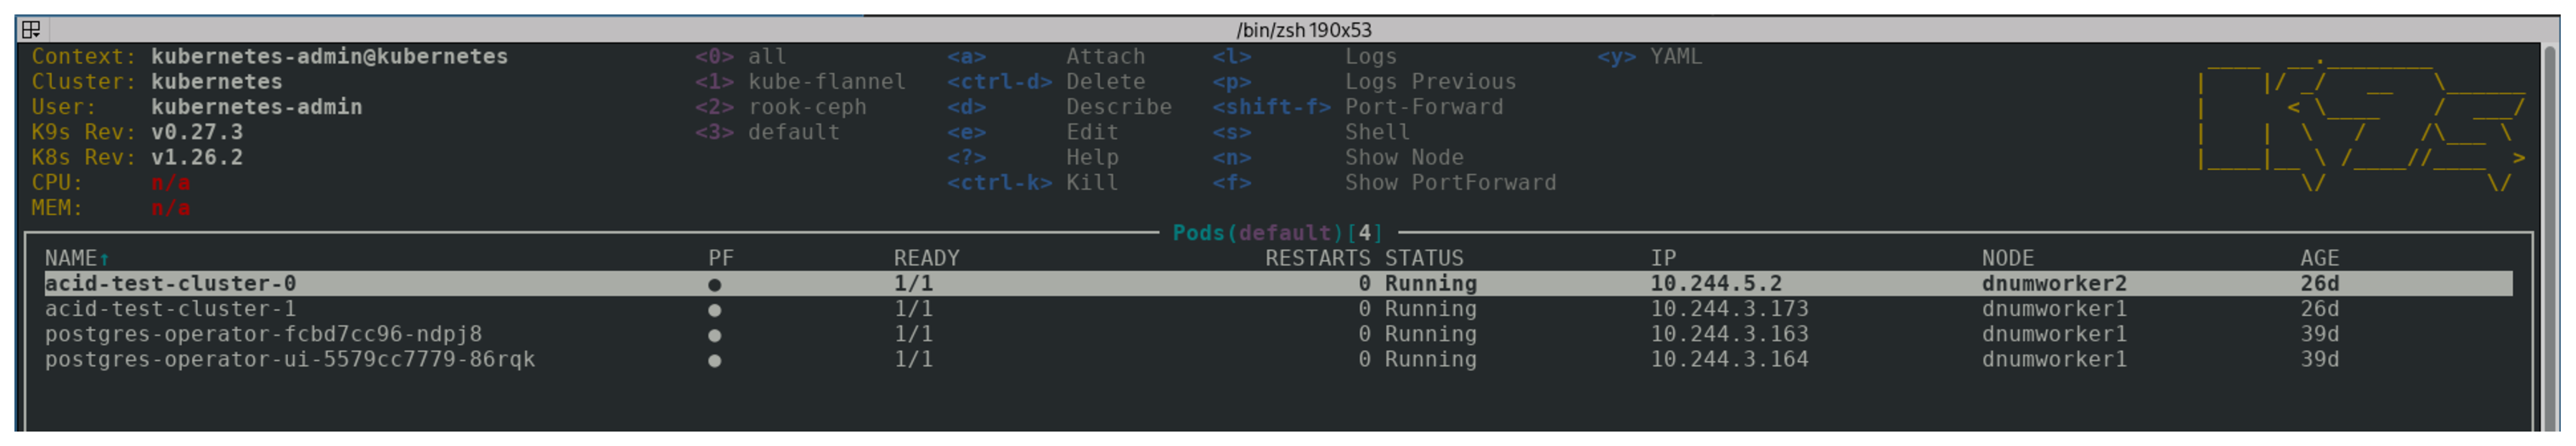
\includegraphics[angle=0, width=0.5\textwidth]{pod-default-ns.eps}
\end{center}
\end{figure}

\end{frame}

%%%%%%%%%%%%%%%%%%%%%%%%%%%%%%%%%%%%%%%%%%%%%%%%%%%%%%%%%%%%%%%%%%%%%%%%%%%%%%%%

\begin{frame}[fragile]{Pods du namespace kube-system}

\begin{tiny}
\begin{Verbatim}[commandchars=\\\{\}]
linagora@debian-cp:~$ kubectl get pods -n kube-system
NAME                                READY   STATUS    RESTARTS           AGE
coredns-787d4945fb-8ph9v            1/1     Running   0                  40d
coredns-787d4945fb-9jrzs            1/1     Running   0                  40d
etcd-debian-cp                      1/1     Running   158                41d
kube-apiserver-debian-cp            0/1     Running   4968 (13m ago)     41d
kube-controller-manager-debian-cp   1/1     Running   4161 (8m26s ago)   41d
kube-proxy-4mfn8                    1/1     Running   0                  33d
kube-proxy-9h4c6                    1/1     Running   0                  27d
kube-proxy-9j47t                    1/1     Running   0                  33d
kube-proxy-s78vx                    1/1     Running   0                  33d
kube-proxy-wpwt4                    1/1     Running   0                  40d
kube-proxy-xjs5q                    1/1     Running   1 (33d ago)        41d
kube-scheduler-debian-cp            1/1     Running   2848 (6m20s ago)   41d
\end{Verbatim}
\end{tiny}

\begin{figure}
\begin{center}
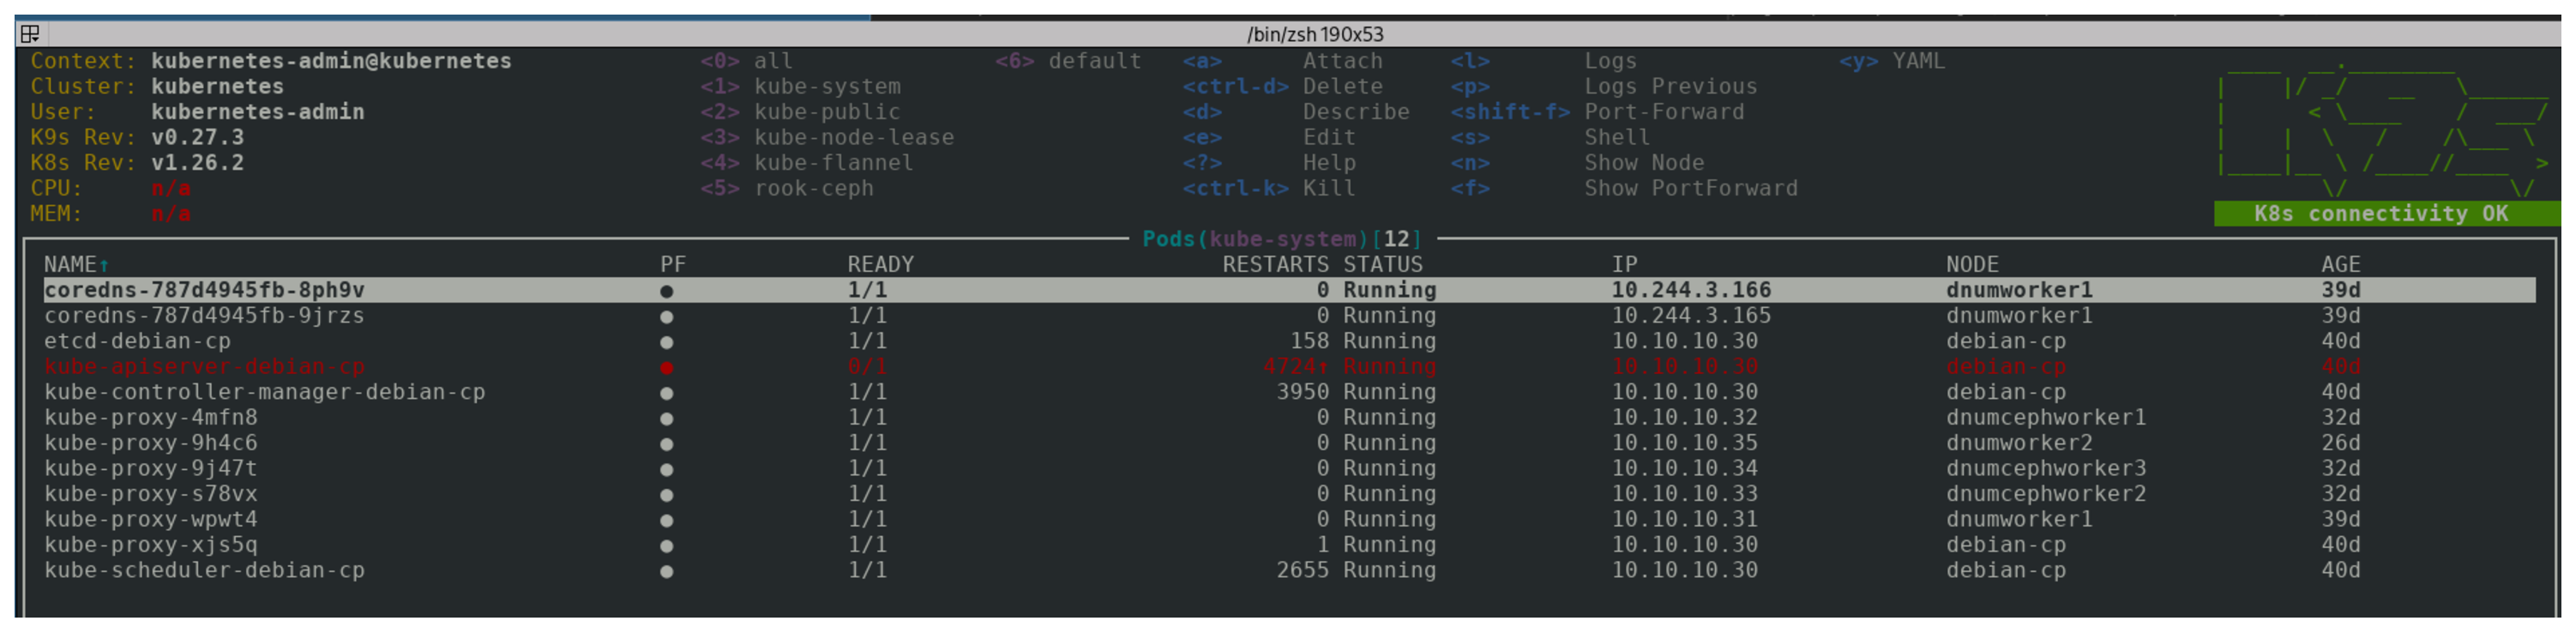
\includegraphics[angle=0, width=0.5\textwidth]{pod-kube-system.eps}
\end{center}
\end{figure}

\end{frame}

%%%%%%%%%%%%%%%%%%%%%%%%%%%%%%%%%%%%%%%%%%%%%%%%%%%%%%%%%%%%%%%%%%%%%%%%%%%%%%%%

\begin{frame}[fragile]{Pods du namespace kube-flannel}

\begin{tiny}
\begin{Verbatim}[commandchars=\\\{\}]
linagora@debian-cp:~$ kubectl get pods -n kube-flannel                                                                                                                                        
NAME                    READY   STATUS    RESTARTS      AGE                                                                                                                                   
kube-flannel-ds-5nw2j   1/1     Running   0             33d                                                                                                                                   
kube-flannel-ds-5xwsm   1/1     Running   0             40d                                                                                                                                   
kube-flannel-ds-8vkg9   1/1     Running   1 (33d ago)   40d                                                                                                                                   
kube-flannel-ds-pv6ss   1/1     Running   0             27d                                                                                                                                   
kube-flannel-ds-trbz9   1/1     Running   0             33d                                                                                                                                   
kube-flannel-ds-wmzz2   1/1     Running   0             33d
\end{Verbatim}
\end{tiny}

\begin{figure}
\begin{center}
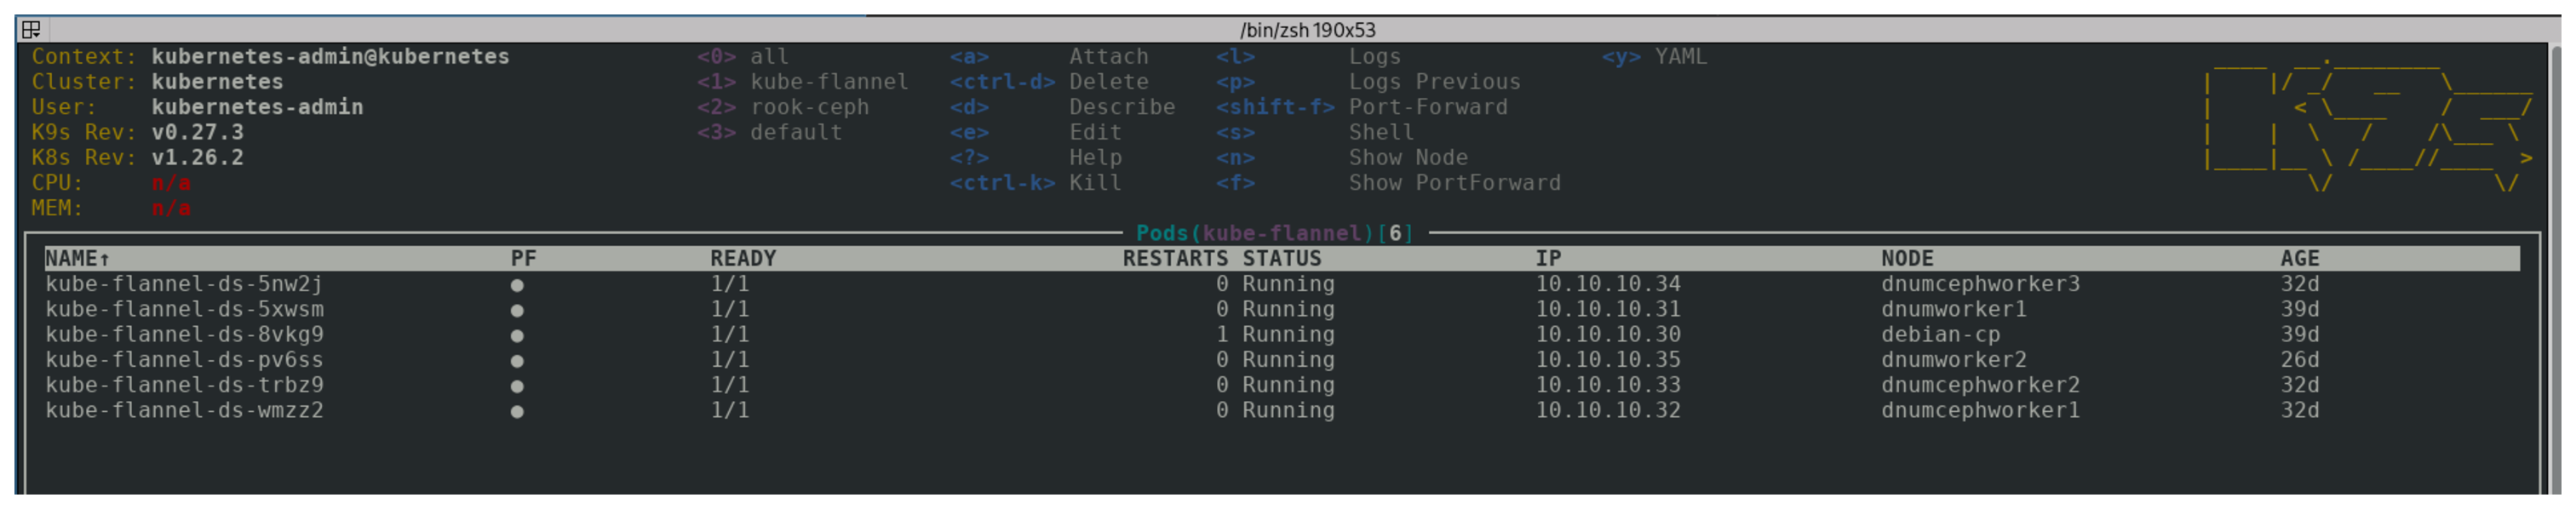
\includegraphics[angle=0, width=0.5\textwidth]{flannel.eps}
\end{center}
\end{figure}

\end{frame}

%%%%%%%%%%%%%%%%%%%%%%%%%%%%%%%%%%%%%%%%%%%%%%%%%%%%%%%%%%%%%%%%%%%%%%%%%%%%%%%%

\begin{frame}[fragile,shrink=0.9]{Pods du namespace rook-ceph}

\begin{tiny}
\begin{Verbatim}[commandchars=\\\{\}]
linagora@debian-cp:~$ kubectl get pods -n rook-ceph
NAME                                                        READY   STATUS                 RESTARTS           AGE
csi-cephfsplugin-9nbts                                      2/2     Running                1 (27d ago)        27d
csi-cephfsplugin-bpxlw                                      2/2     Running                0                  33d
csi-cephfsplugin-jd5x8                                      2/2     Running                0                  33d
csi-cephfsplugin-mddkf                                      2/2     Running                0                  33d
csi-cephfsplugin-nrmfz                                      2/2     Running                0                  33d
csi-cephfsplugin-provisioner-84cc595b78-9mml4               5/5     Running                6008 (2m44s ago)   33d
csi-cephfsplugin-provisioner-84cc595b78-9twnq               5/5     Running                2171               33d
csi-rbdplugin-92zlq                                         2/2     Running                0                  33d
csi-rbdplugin-c95w7                                         2/2     Running                0                  33d
csi-rbdplugin-pk57s                                         2/2     Running                1 (27d ago)        27d
csi-rbdplugin-provisioner-6f6b6b8cd6-4c8jd                  1/5     CreateContainerError   1344               33d
csi-rbdplugin-provisioner-6f6b6b8cd6-gw6bm                  1/5     CreateContainerError   4465               33d
csi-rbdplugin-srtfz                                         2/2     Running                0                  33d
csi-rbdplugin-v6gqm                                         2/2     Running                0                  33d
rook-ceph-crashcollector-dnumcephworker1-7845bb8ff-vs9fx    1/1     Running                0                  32d
rook-ceph-crashcollector-dnumcephworker2-75cdf95dcd-n5xsz   1/1     Running                0                  33d
rook-ceph-crashcollector-dnumcephworker3-6fddb6cd9-x45w5    1/1     Running                1 (8d ago)         32d
rook-ceph-mgr-a-c5db58dff-hvsp9                             3/3     Running                1487 (6d6h ago)    33d
rook-ceph-mgr-b-7bbfd88c8b-wh4ww                            2/3     CreateContainerError   944                22d
rook-ceph-mon-a-75cf9ccddc-b2jgc                            2/2     Running                1163               33d
rook-ceph-mon-b-78d6586d5-qss4z                             1/2     CreateContainerError   701 (19d ago)      19d
rook-ceph-mon-c-64dcb4c86c-wz8sg                            2/2     Running                1755               33d
rook-ceph-operator-cf4f7dfd4-6tm6p                          1/1     Running                0                  32d
rook-ceph-osd-0-57d9b8db4d-d6dhr                            1/2     CreateContainerError   484                32d
rook-ceph-osd-1-74698f77fd-6n2mh                            1/2     Running                529                32d
rook-ceph-osd-2-5cc486467c-lhm47                            1/2     Running                1116 (49m ago)     32d
rook-ceph-osd-prepare-dnumcephworker1-rnk78                 0/1     Completed              0                  21d
rook-ceph-osd-prepare-dnumcephworker3-42rxv                 0/1     Completed              0                  21d
rook-ceph-tools-7c4b8bb9b5-pxk67                            1/1     Running                0                  33d
\end{Verbatim}
\end{tiny}

\begin{figure}
\begin{center}
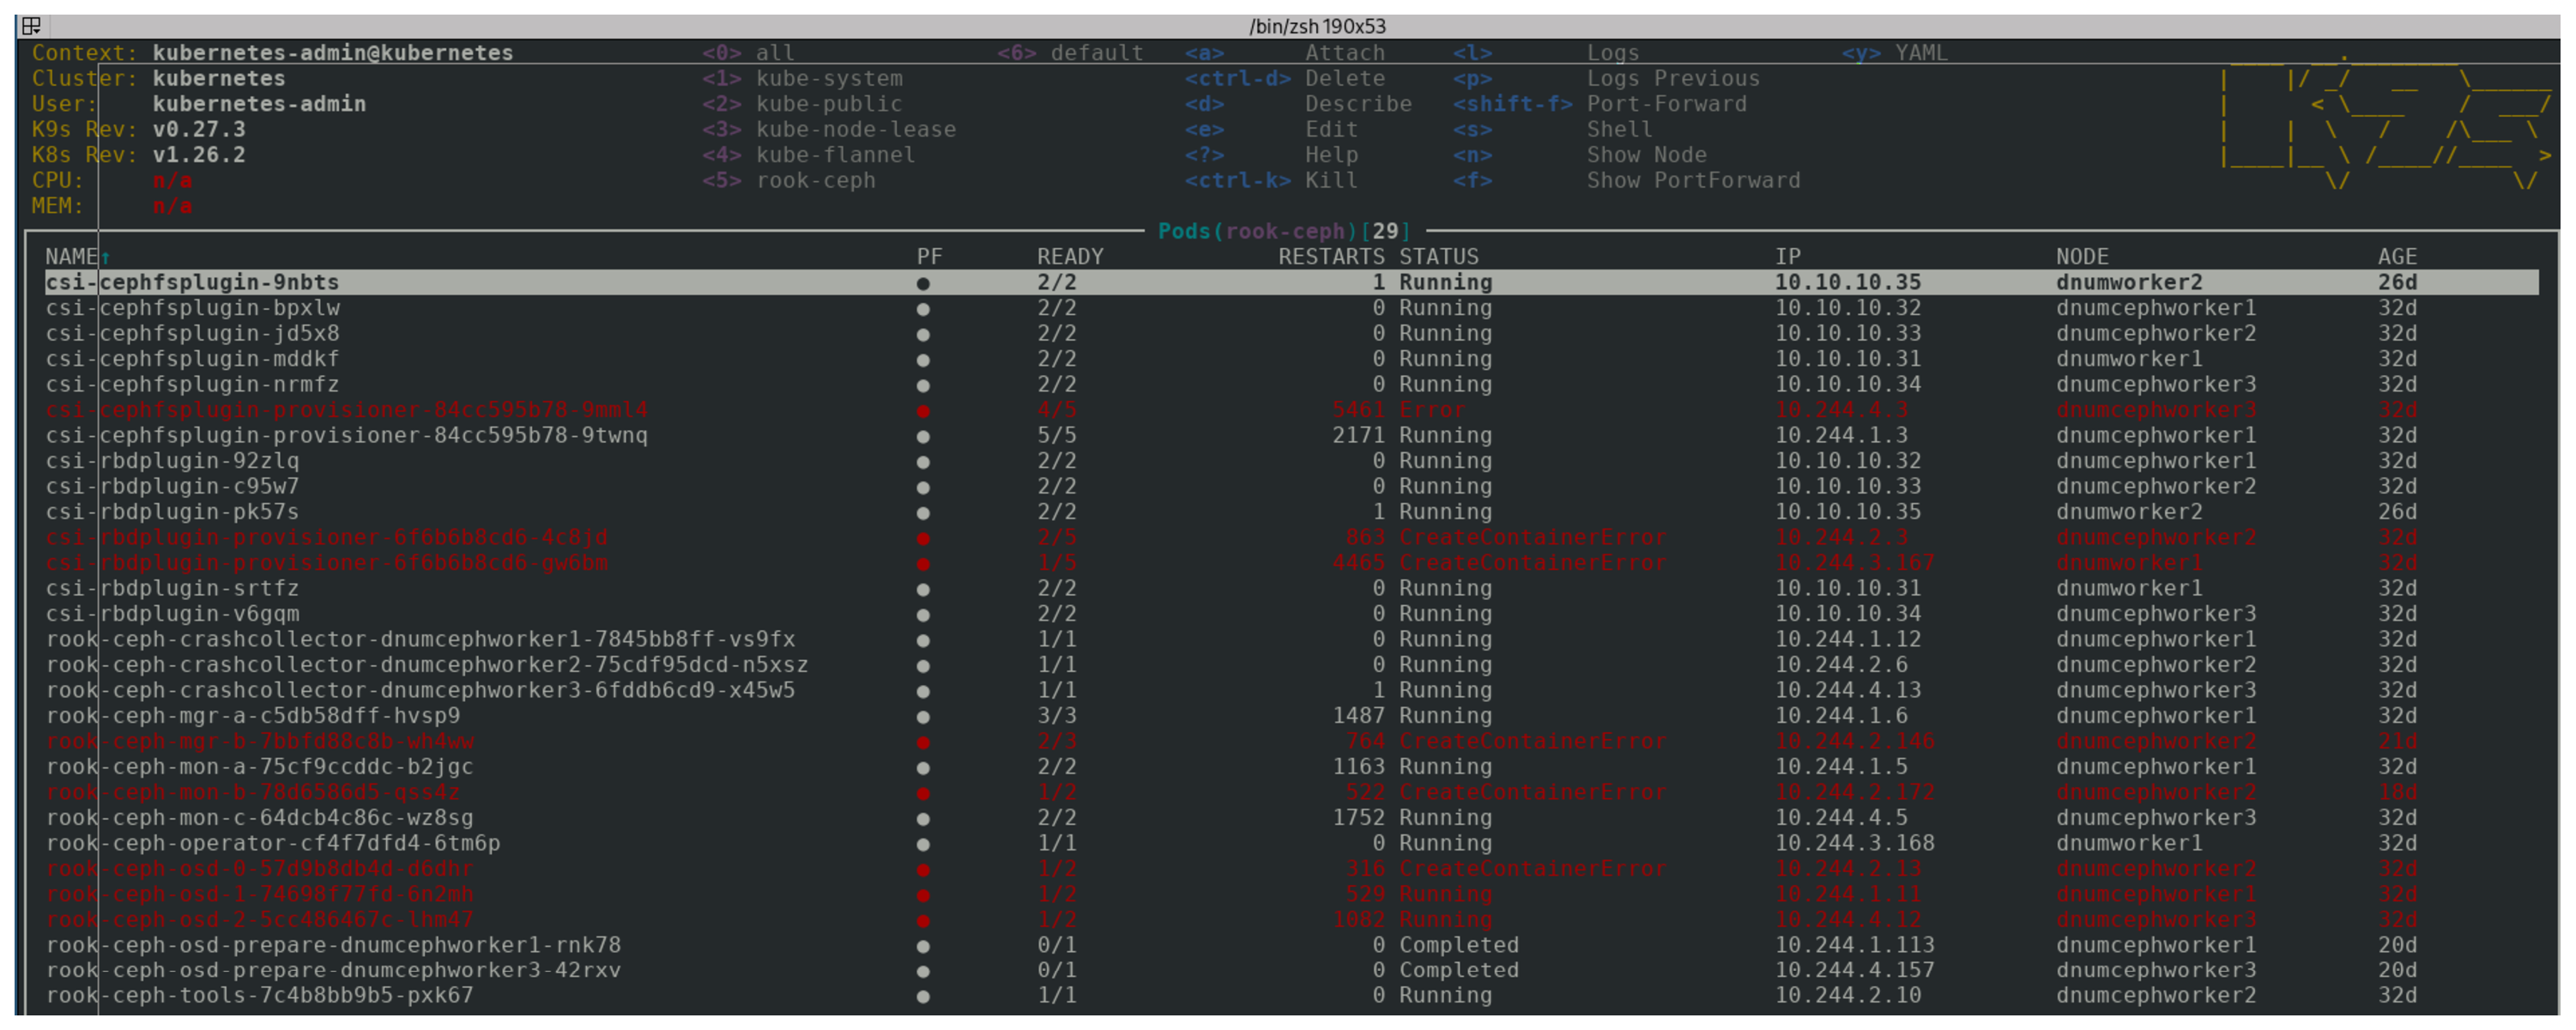
\includegraphics[angle=0, width=0.5\textwidth]{pod-rook-ceph.eps}
\end{center}
\end{figure}

\end{frame}

%%%%%%%%%%%%%%%%%%%%%%%%%%%%%%%%%%%%%%%%%%%%%%%%%%%%%%%%%%%%%%%%%%%%%%%%%%%%%%%%

\begin{frame}[fragile]{Déploiement du n{\oe}ud \textbf{worker}}

   Sur chacun des 2 workers, il est nécessaire de déployer:
   \begin{itemize}
      \item le runtime containerd de Docker
      \item les commandes kubectl, kubeadm et kubelet
      \item l'activation des modules kernel overlay et br\_netfilter
      \item l'activation des fonctions bridge/iptables et forward du kernel
      \item le paramétrage de containerd
   \end{itemize}

\end{frame}

%%%%%%%%%%%%%%%%%%%%%%%%%%%%%%%%%%%%%%%%%%%%%%%%%%%%%%%%%%%%%%%%%%%%%%%%%%%%%%%%

\begin{frame}[shrink=8,fragile]{Ajout du n{\oe}ud \textbf{worker} dans le cluster k8s - \textbf{join}}

   L'opération qui permet au n{\oe}ud worker de rejoindre le cluster s'appelle le join.\\
   La syntaxe de cette commande est obtenue en lançant la commande suivante sur le control plane avec l'utilisateur root:

\begin{tiny}
\begin{Verbatim}[commandchars=\&\@\@]
# kubeadm token create --print-join-command
kubeadm join 10.10.10.30:6443 \
--token ilfbgc.8xco4svm5pnxkfbj \
--discovery-token-ca-cert-hash sha256:73bf45619ae0051d4ff810328d1dadc18e6a5966c95d3c4ec76275b89a934595 
\end{Verbatim}
\end{tiny}

\end{frame}

%%%%%%%%%%%%%%%%%%%%%%%%%%%%%%%%%%%%%%%%%%%%%%%%%%%%%%%%%%%%%%%%%%%%%%%%%%%%%%%%

\begin{frame}[fragile]{Lancement du join sur chacun des workers}

Sur chacun des workers, le lancement de la commande join produit le résultat suivant:
\begin{tiny}
\begin{Verbatim}[commandchars=\&\@\@]
# kubeadm join 10.10.10.30:6443 \
--token 6pia7c.n6u8pbm7yjl6nnr8 \
--discovery-token-ca-cert-hash sha256:f6d45602ea75c7659dc91f661d19e97e6817e2847e4e5d0047880b871317a145
[preflight] Running pre-flight checks
[preflight] Reading configuration from the cluster...
[preflight] FYI: You can look at this config file with 'kubectl -n kube-system get cm kubeadm-config -o yaml'
W0315 16:31:41.445771    6266 configset.go:78] Warning: No kubeproxy.config.k8s.io/v1alpha1 config is loaded. Continuing without it: configmaps "kube-proxy" is forbidden: User "system:bootstrap:6pia7c" cannot get resource "configmaps" in API group "" in the namespace "kube-system"
[kubelet-start] Writing kubelet configuration to file "/var/lib/kubelet/config.yaml"
[kubelet-start] Writing kubelet environment file with flags to file "/var/lib/kubelet/kubeadm-flags.env"
[kubelet-start] Starting the kubelet
[kubelet-start] Waiting for the kubelet to perform the TLS Bootstrap...

This node has joined the cluster:
* Certificate signing request was sent to apiserver and a response was received.
* The Kubelet was informed of the new secure connection details.

Run 'kubectl get nodes' on the control-plane to see this node join the cluster.
\end{Verbatim}
\end{tiny}

La commande suivante permet de vérifier le résultat du join:
\begin{tiny}
\begin{Verbatim}[commandchars=\&\@\@]
$ kubectl get nodes
NAME          STATUS     ROLES           AGE   VERSION
debian-cp     NotReady   control-plane   15h   v1.26.2
dnumworker1   NotReady   <none>          53s   v1.26.2

\end{Verbatim}
\end{tiny}

\end{frame}

%%%%%%%%%%%%%%%%%%%%%%%%%%%%%%%%%%%%%%%%%%%%%%%%%%%%%%%%%%%%%%%%%%%%%%%%%%%%%%%%

\begin{frame}[shrink=8,fragile]{Terminologie du stockage dans k8s}

\begin{itemize}
   \item Le stockage permanent des données s'appuie les volumes persistants (PV) (\url{https://kubernetes.io/docs/concepts/storage/persistent-volumes/})
   \item Un PV est un espace de stockage mis à disposition par k8s.
   \item Il peut être alloué manuellement ou dynamiquement par l'intermédiaire des storage class (\url{https://kubernetes.io/docs/concepts/storage/storage-classes/})
   \item Les PV sont l'équivalent d'un node dans un cluster.
   \item Les persistentVolumeClaim (PVC) sont l'équivalent d'un pod.
\end{itemize}

\end{frame}

%%%%%%%%%%%%%%%%%%%%%%%%%%%%%%%%%%%%%%%%%%%%%%%%%%%%%%%%%%%%%%%%%%%%%%%%%%%%%%%%

\begin{frame}[fragile]{Déploiement du stockage - \textbf{Rook Ceph}}

\begin{itemize}
   \item Le storage class sur lequel s'appuie l'opérateur PostgreSQL est Ceph
   \item L'opérateur k8s \textbf{Rook Ceph} facilite le déploiement de Ceph
   \item Le déploiement s'appuie sur le lien \url{https://rook.io/docs/rook/v1.9/quickstart.html}
   \item La version de l'opérateur utilisée est la v1.9
   \item Elle supporte les versions k8s v1.17+
\end{itemize}

\end{frame}

%%%%%%%%%%%%%%%%%%%%%%%%%%%%%%%%%%%%%%%%%%%%%%%%%%%%%%%%%%%%%%%%%%%%%%%%%%%%%%%%

\begin{frame}[fragile]{Prérequis au déploiement de l'opérateur - \textbf{Rook Ceph}}

\begin{itemize}
   \item Le déploiement de l'opérateur scanne l'ensemble des noeuds de stockage pour vérifier la présence de:
   \begin{itemize}
      \item des devices bruts (sans partitions ou filesystems formattés)
      \item des partitions brutes (sans filesystems formattés)
      \item les volumes physiques initialisés par LVM
   \end{itemize}
\end{itemize}

L'exemple ci-dessous indique comment vérifier la disponibilité d'espace pour l'opérateur Rook Ceph:

\begin{tiny}
\begin{Verbatim}[commandchars=\\\{\}]
lsblk -f

    NAME                  FSTYPE      LABEL UUID                                   MOUNTPOINT
    vda
    |-vda1                LVM2_member       >eSO50t-GkUV-YKTH-WsGq-hNJY-eKNf-3i07IB
     |-ubuntu--vg-root   ext4              c2366f76-6e21-4f10-a8f3-6776212e2fe4   /
     |-ubuntu--vg-swap_1 swap              9492a3dc-ad75-47cd-9596-678e8cf17ff9   [SWAP]
    vdb
\end{Verbatim}
\end{tiny}

\end{frame}

%%%%%%%%%%%%%%%%%%%%%%%%%%%%%%%%%%%%%%%%%%%%%%%%%%%%%%%%%%%%%%%%%%%%%%%%%%%%%%%%

\begin{frame}[fragile]{Prérequis au déploiement de l'opérateur - \textbf{Rook Ceph}}

\begin{itemize}
   \item Dans l'exemple précédent, si la colonne \textit{FSTYPE} est renseignée, cela indique la présence d'un filesystem
   \item La partition vdb n'est pas formatée avec un filesystem: elle est donc utilisable par l'opérateur Rook Ceph
   \item Le paquet \textbf{lvm2} est une dépendance importante de Rook Ceph
\end{itemize}

\end{frame}

%%%%%%%%%%%%%%%%%%%%%%%%%%%%%%%%%%%%%%%%%%%%%%%%%%%%%%%%%%%%%%%%%%%%%%%%%%%%%%%%

\begin{frame}[fragile]{Déploiement de l'opérateur \textbf{Rook Ceph}}

\begin{tiny}
\begin{Verbatim}[commandchars=\\\{\}]
$ git clone --single-branch --branch v1.9.2 https://github.com/rook/rook.git
cd rook/deploy/examples
kubectl create -f crds.yaml -f common.yaml -f operator.yaml
kubectl create -f cluster.yaml
\end{Verbatim}
\end{tiny}

\begin{itemize}
   \item Une fois le cluster est opérationnel, il devient possible de créer:
   \begin{itemize}
      \item stockage bloc
      \item stockage objet
      \item stockage fichier
   \end{itemize}
\end{itemize}

\end{frame}

%%%%%%%%%%%%%%%%%%%%%%%%%%%%%%%%%%%%%%%%%%%%%%%%%%%%%%%%%%%%%%%%%%%%%%%%%%%%%%%%

\begin{frame}[fragile]{Vérification de l'opérateur \textbf{Rook Ceph}}

\begin{tiny}
\begin{Verbatim}[commandchars=\\\{\}]
# verify the rook-ceph-operator is in the `Running` state before proceeding
kubectl -n rook-ceph get pod
\end{Verbatim}
\end{tiny}

\end{frame}

%%%%%%%%%%%%%%%%%%%%%%%%%%%%%%%%%%%%%%%%%%%%%%%%%%%%%%%%%%%%%%%%%%%%%%%%%%%%%%%%

\begin{frame}[fragile]{Le contrôleur d'admission (Admission Controller) - \textbf{Rook Ceph}}

\begin{itemize}
   \item Il est recommandé de déployer le contrôleur d'admission: il permet de vérifier que Rook est correctement paramétré grâce aux réglages des Customer Resources (CR)
   \item L'Admission Controller intercepte les requêtes à destination de l'API k8s avant l'objet persistant après les phases d'authentification et d'autorisation
   \item Pour installer l'Admission Controller, lancer les requêtes suivantes:

\begin{tiny}
\begin{Verbatim}[commandchars=\\\{\}]
kubectl apply -f https://github.com/jetstack/cert-manager/releases/download/v1.7.1/cert-manager.yaml
\end{Verbatim}
\end{tiny}

\end{itemize}

\end{frame}

%%%%%%%%%%%%%%%%%%%%%%%%%%%%%%%%%%%%%%%%%%%%%%%%%%%%%%%%%%%%%%%%%%%%%%%%%%%%%%%%

\begin{frame}[fragile]{Affichage des storage class déployés}

\begin{tiny}
\begin{Verbatim}[commandchars=\\\{\}]
linagora@debian-cp:~$ kubectl get storageclass
NAME              PROVISIONER                    RECLAIMPOLICY   VOLUMEBINDINGMODE      ALLOWVOLUMEEXPANSION   AGE
local-storage     kubernetes.io/no-provisioner   Delete          WaitForFirstConsumer   false                  12d
rook-ceph-block   rook-ceph.rbd.csi.ceph.com     Delete          Immediate              true                   5d23h
\end{Verbatim}
\end{tiny}

\end{frame}

%%%%%%%%%%%%%%%%%%%%%%%%%%%%%%%%%%%%%%%%%%%%%%%%%%%%%%%%%%%%%%%%%%%%%%%%%%%%%%%%

\begin{frame}[fragile]{Déploiement de l'opérateur \textbf{PostgreSQL} de Zalando}

TODO

\end{frame}

%%%%%%%%%%%%%%%%%%%%%%%%%%%%%%%%%%%%%%%%%%%%%%%%%%%%%%%%%%%%%%%%%%%%%%%%%%%%%%%%

\begin{frame}[fragile]{Répartitions des pods \textbf{PostgreSQL} sur les n{\oe}uds worker}

TODO

\end{frame}

%%%%%%%%%%%%%%%%%%%%%%%%%%%%%%%%%%%%%%%%%%%%%%%%%%%%%%%%%%%%%%%%%%%%%%%%%%%%%%%%
